\chapter{System Design}
\label{chapter:design}

\section{Overview}
    \begin{table}[h]
    \centering
    % [] ��ܦb list of tables ����r
    % {} ��ܦb����W�誺��r
    \caption[Notations]{Notations}
    \label{table:notation}
    \begin{tabular}{lll}
    \toprule[1.1pt]
    Notation   & Description\\
    \midrule[1.1pt]
    \multirow{1}{*}{\(C_i\)} & Customer / User\\
    \midrule
    \multirow{1}{*}{\(Org_i\)} & Organization\\
    \midrule
    \multirow{1}{*}{\(RA\)} & Regulatory Authority\\
    \midrule
    \multirow{1}{*}{\(D_{ij}\)} & Data of \(C_i\) in \(Org_j\)\\
    \midrule
    \multirow{1}{*}{\({TSP}_i\)} & Third-party Service Provider\\
    \midrule
    \multirow{1}{*}{\({Acc}_{ij}\)} & \(Org_j\) Account of \(C_i\)\\
    \midrule
    \multirow{1}{*}{\({ID}_i\)} & Identification card number of \(C_i\)\\
    \midrule
    \multirow{1}{*}{\({Add}_i\)} & Ethereum address of i\\
    \midrule
    \multirow{1}{*}{\({Pri}_i\)} & Private key of \({Add}_i\)\\
    \midrule
    \multirow{1}{*}{\({DI}_i\)} & Digital Identity of \(C_i\)\\
    \midrule
    \multirow{1}{*}{\({R}_{ijk}\)} & Access right of \({TSP}_i\) to access \({Org}_j\) with \(C_k\) consent\\
    \midrule
    \multirow{1}{*}{\({ACMgr}_i\)} & Access Control Manager contract of \(C_i\) \\
    \midrule
    \multirow{1}{*}{\({OMgr}\)} & Organization contract \\
    \midrule
    \multirow{1}{*}{\({N}\)} & Nonce \\
    \bottomrule[1.1pt]
    \end{tabular}
    \end{table}
    \newpage    

    \begin{figure}[htb]
        \centering
        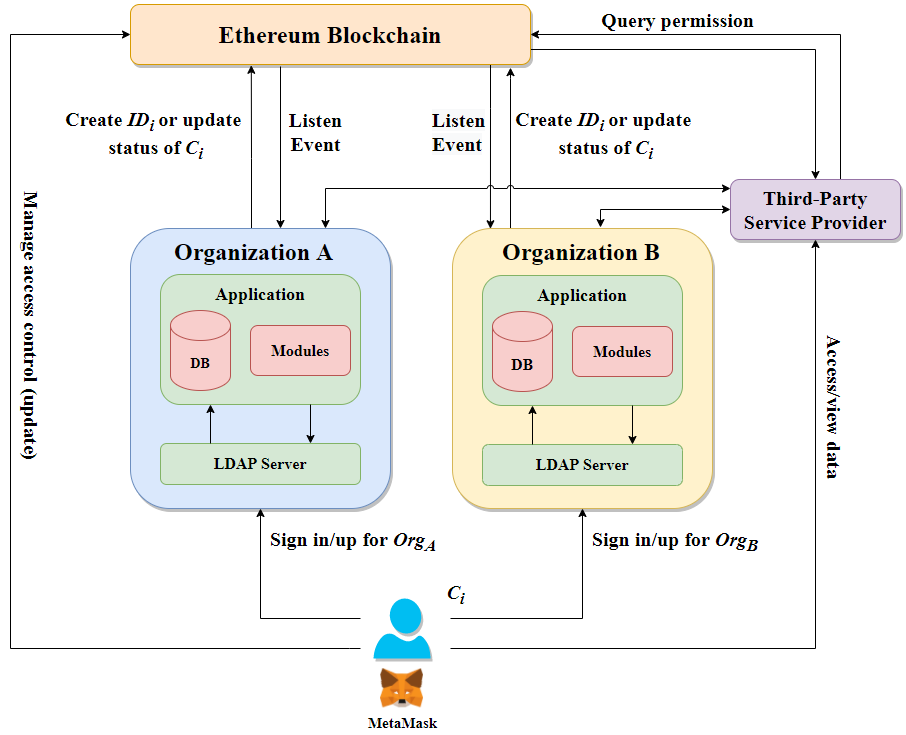
\includegraphics[height=!,width=1\linewidth,keepaspectratio=true]{figures/system_architecture.png}
        \caption{{\footnotesize System Architecture}}
        \label{fig:system_architecture}
    \end{figure}
    The architecture of our system is given in figure~\ref{fig:system_architecture}. Our proposed system solved the account integration and identity verification. And it can apply to various scenarios which need data sharing and distributed access control management such as open banking, medical records, and academic records. At the initial stage, each \(Org\) or \(TSP\) gets the exclusive \(Add\) and the corresponding \(Pri\) to take part in our open banking ecosystem. They must put the safety of \(Pri\) first and be careful; otherwise, identity theft may occur. Our system employs the hash algorithm Keccak-256 to hash \(C_i\)'s identity information, i.e., \(ID_i\). This system records the hash value in the blockchain to represent \(C_i\)'s identity instead of storing \(ID_i\). There are several parties in our system: blockchain network, organization, third-party service provider, and user. The interpretation of these parties is stated as following:\par

    \begin{itemize}
        \item \textbf{Blockchain network:} The Ethereum blockchain network is used to store the user's \(DI\) and data access rights and deploy smart contracts, including identity creation and storage. Every node on blockchain has a copy of the ledger and ensures data on the blockchain cannot be tampered with. With decentralized technology, the management of data access rights doesn't have any governing authority to monitor. There have two kinds of contracts to realize that account integration and access manager, detailed in Sect.~\ref{chapter:implementation}.  
        \item \textbf{Organization:} A set of organizations within an ecosystem, identified by the \(Add\) and IP addresses. Each organization represents an independent system, it owns membership software that provides an organization with functionality such as storing and editing member information. The organization not only provides services to customers depend on applications, but also collects user data by using a database. In this paper, organizations provide an interface that users decide to share data.
        \begin{itemize}[noitemsep]
            \item $DB_j = \{D_{1j}, D_{2j}, ..., D_{nj}\}$: Database of $Org_j$ is used to store customer data and only owner of data can decide which $TSP$ can access. 
            \item Because the organization $Org_j$ maintains membership software, it will provide the user $C_i$ a regular account $Acc_{ij}$. In the appilcation of $Org_j$, the user $C_i$ can access their data $D_{ij}$.
        \end{itemize}
        \item \textbf{Third-party service provider:} The third-party service provider can be any organization or entity that performs financial services to customer. In this paper, we assume that TSP doesn't manage membership software and they retrieve customer data through blockchain technology.
        \begin{itemize}[noitemsep]
            \item The aim of the $TSP$ is for collect data of $C_i$ from organizations $\{Org_1, Org_2, ..., Org_n\}$ if the organization owns the data of $C_i$ and $TSP$ gets the permission.
            \item When the permission is revoked by triggering smart contract, the access data request is regarded as invalid even if the token exists and it is not out of date.
        \end{itemize}
        \item \textbf{User:} A user owns an organization account and wants to participate in our proposed system. After registering an organization account, the user first needs to pass identity card authentication. Due to the digital identity is unique and important on the smart contract, the organization takes responsibility for ensuring the correct identification card number and the safety of user's personal data. Besides, the user should generate the Ethereum account themself through Metamask.
    \end{itemize}

    \newpage    
\section{Scenario}
    \begin{figure}[htb]
        \centering
        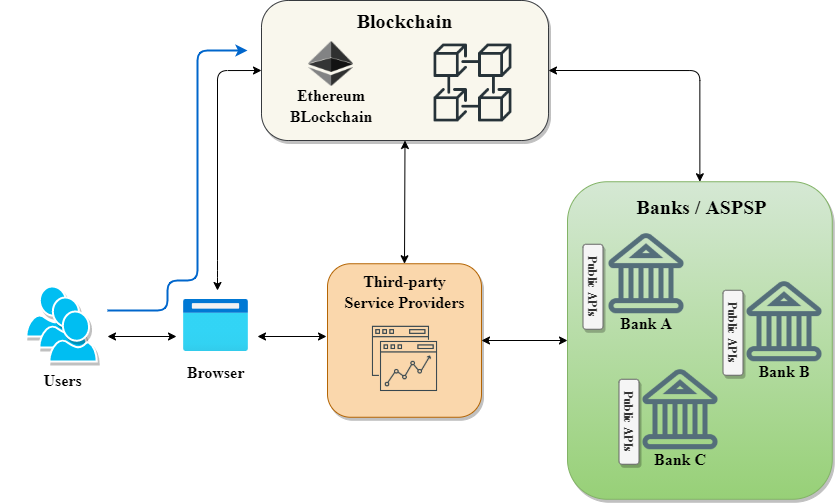
\includegraphics[height=!,width=1\linewidth,keepaspectratio=true]{figures/system architecture-banks.png}
        \caption{{\footnotesize Relation between open banking roles}}
        \label{fig:relation}
    \end{figure}
        From the user perspective, our proposed system provides a single digital identity \(DI_i\) and access control. The access control for data sharing is constructed using smart contracts. So when banks disclose user's personal data to TSP, banks must have the user's consent through call specific user's smart contract. \par
        In order to apply our proposed system to open banking ecosystem, we have three clearly defined roles: Customer (User), Financial institution, and Third-party services provider. Figure~\ref{fig:relation} gives an overview of our proposed system. It shows the relation between these roles and includes workflows, detailed in Sect.~\ref{ssec:workflow} Each customer interacts with Blockchain by using MetaMask, they not only login with MetaMask but also manage their own access manager contract. That's why customers can allow the specific party to access their data.\par
        The user can specify the data attribute, source, destination through the smart contract to decentralized access control. And the user also can revoke access rights while he/she doesn't need the service that TSP provides.\par
        
\section{Workflow} \label{ssec:workflow}
    \subsection{Identity verification}
    \begin{figure}[htb]
        \centering
        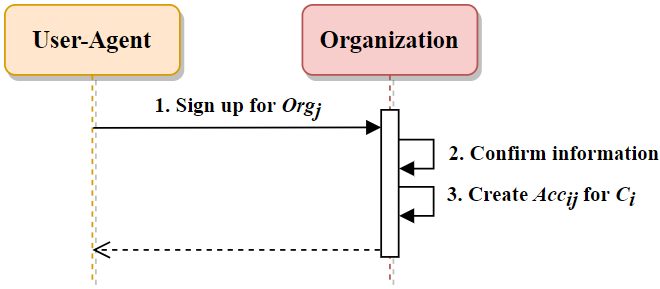
\includegraphics[height=!,width=0.8\linewidth,keepaspectratio=true]{figures/account_creation.png}
        \caption{{\footnotesize Account creation flow}}
        \label{fig:accountCreation}
    \end{figure}
    User registration is commonly used by many companies or any online service which record user data. Although in recent years there has been an increase in social login, the sign-up for social media is still necessary. Figure~\ref{fig:accountCreation} shows the flow for the user who visits the application (e.g., bank's website) and completes a signup form as shown in Table~\ref{table:signup}. The identification card number of the form is especially important for identity because it can be used to establish a digital identity on the blockchain. In this paper, we assume every organization should have its own membership software such as LDAP . And every user has multiple accounts, their personal information and data generated through organization service are belong to the organization themself.\par
    
    \begin{table}[h]
    \centering
    % [] ��ܦb list of tables ����r
    % {} ��ܦb����W�誺��r
    \caption[Sign-up form used in each organization]{Sign-up form used in each organization}
    \label{table:signup}
    \begin{tabular}{lll}
    \toprule[1.1pt]
    Fields   & Description & required\\
    \midrule[1.1pt]
    \multirow{1}{*}{username} & Username as login account & Yes\\
    \midrule
    \multirow{1}{*}{password} & The password of the account & Yes \\
    \midrule
    \multirow{1}{*}{email} & User's email & No \\
    \midrule
    \multirow{1}{*}{phone} & User's phone & No \\
    \midrule
    \multirow{1}{*}{id card number} & Identification card number & No \\
    \bottomrule[1.1pt]
    \end{tabular}
    \end{table}
    \newpage

    Customers should remember their username and password pairs for different sites. The username of the form is the account \(Acc\) for log in to \(Org_j\), many real-world applications already adopt this scheme to build their membership system. An individual customer \(C_i\) of the real world usually has many accounts \(\{Acc_{i1}, Acc_{i2}, ..., Acc_{in}\}\), those accounts are independent of each other under the current ecosystem.\par

    \begin{figure}[htb]
        \centering
        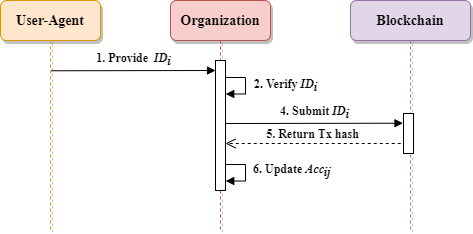
\includegraphics[height=!,width=0.8\linewidth,keepaspectratio=true]{figures/identity_verification.png}
        \caption{{\footnotesize Identity verification flow}}
        \label{fig:identityVerification}
    \end{figure}
    Figure~\ref{fig:identityVerification} shows the flow that an individual customer applies for real-name authentication. Participating in existing blockchain-based open banking ecosystems requires real-name authentication in order to prevent identity theft and avoid duplicate data. \par
    In the first step, every user who wants to enable blockchain-based functionality carries their own personal identification card. After verifying by the staff of the bank, the \(ID_i\) will be submitted to blockchain by invoking \(OMgr\)'s function, and then update the user's account status for pass authentication.\par
    In this paper, we assume that organizations or banks are trustworthy, they won't submit fake information. But if they are the malicious attacker, they only submit the wrong \(ID_i\) and create an empty \(DI_i\) on blockchain without harming the user's right or revealing personal data.

    \newpage
    \subsection{Account binding \& unbinding}
    \begin{figure}[htb]
        \centering
        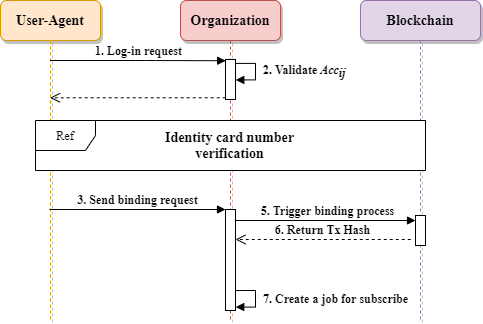
\includegraphics[height=!,width=0.8\linewidth,keepaspectratio=true]{figures/account_binding.png}
        \caption{{\footnotesize Account binding flow}}
        \label{fig:accountBinding}
    \end{figure}

    In the account binding process, the user must log in with user's \(Acc\) first and apply for identity verification in person. If users intend to enable third party service, they are required to get a private key and its corresponding Ethereum address. Users can generate their private keys by using MetaMask~\cite{metamask} and store recovery key (seed) in safe location. MetaMask guarantees user's information safety, it won't collect any private keys, addresses, balance and personal information. After retrieving the private key and Ethereum address, users can submit its Ethereum address to the \(Org_i\) server, then the \(Org_i\) check if the address is valid using the smart contract function. Finally, \(Org_i\) triggers the binding process and creates a new job to subscribe to the specific event with a transaction hash. After adding a block of transactions to blockchain, this job will add hashed \(ID_i\) to the status of \(Acc_i\).\par
    Through executing the above process flow, the user identity verification will be confirmed by the bank and the \(DI_i\) will be created by blockchain. After binding Acc with the Ethereum address, users can manage all data access right themselves. This process not only enables distributed access control but also enables third-party login.

    \newpage

    \begin{figure}[htb]
        \centering
        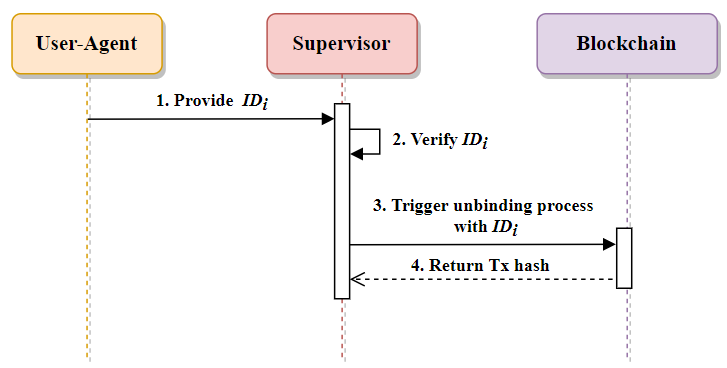
\includegraphics[height=!,width=0.8\linewidth,keepaspectratio=true]{figures/account_unbinding.png}
        \caption{{\footnotesize Account unbinding flow}}
        \label{fig:accountunBinding}
    \end{figure}

    Figure~\ref{fig:accountunBinding} presents that an individual user triggers unbinding account process. To disconnecting a users' \(DI\) from their \(Add\), the unbinding request will be sent to the \(RA\) that is recognized as an impartial third party. If users lose \(Add\)'s private key or intend to bind another \(Add\), they should prepare a new \(Add\) in advance and bring their identity document to \(RA\) to change their binding status.
    \par 
    With this unbinding mechanism, it brings a convenient way to reset and prevent unauthorized transmission of data. Once this process executes successfully and the new mapping is strictly written into the block, the previous address will become invalid for login or any operations. The \(ACMgr\) that the previous address managed stored in the blockchain permanently, and no one can remove this contract except it implements self-destruct function. Even though we can't remove this contract from the blockchain, the attacker is nothing to do. This contract only stores access rights and data attribute names.

    \newpage

    \subsection{Third-party login with Ethereum account}
    \begin{figure}[htb]
        \centering
        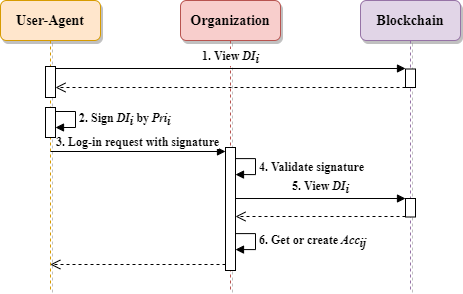
\includegraphics[height=!,width=0.8\linewidth,keepaspectratio=true]{figures/Third_party_login.png}
        \caption{{\footnotesize Third-party login flow}}
        \label{fig:thirdPartyLogin}
    \end{figure}

    In the frontend user-agent, the user utilizes an Ethereum account to retrieve their \(DI_i\) from the blockchain without through a centralized server such as an organization, bank. Then the user signs this \(DI_i\) with MetaMask to generate a digital signature for proof of identity. After that, the server-side validate the authenticity and integrity of this digital signature. Additionally, the server-side also retrieve \(DI_i\) from the blockchain to confirm that the mapping of the Ethereum account and the specific \(DI_i\).
    \par
    The organization in our framework is regarded as service provider with and without the functionality of membership software. In our proposed ecosystem, every organization should support blockchain-based third-party login. For example, if users have enabled the functionality of blockchain, users can use their Ethereum account to log in to any service providers instead of \(Acc_i\) account and password.
    \par 
    The proposed framework supports two kinds of login mechanisms: (1) Regular account login: The user enters the account and password to log in system. The user behavior will not be affected if the user doesn't have Ethereum account. (2) Blockchain-based third-party login: The user can install MetaMask extension then choose third-party login with MetaMask, the server-side will retrieve the corresponding \(Acc\) or create a new one if the user never ever log in.
      
    \newpage
    \subsection{Data sharing}
    \begin{figure}[htb]
        \centering
        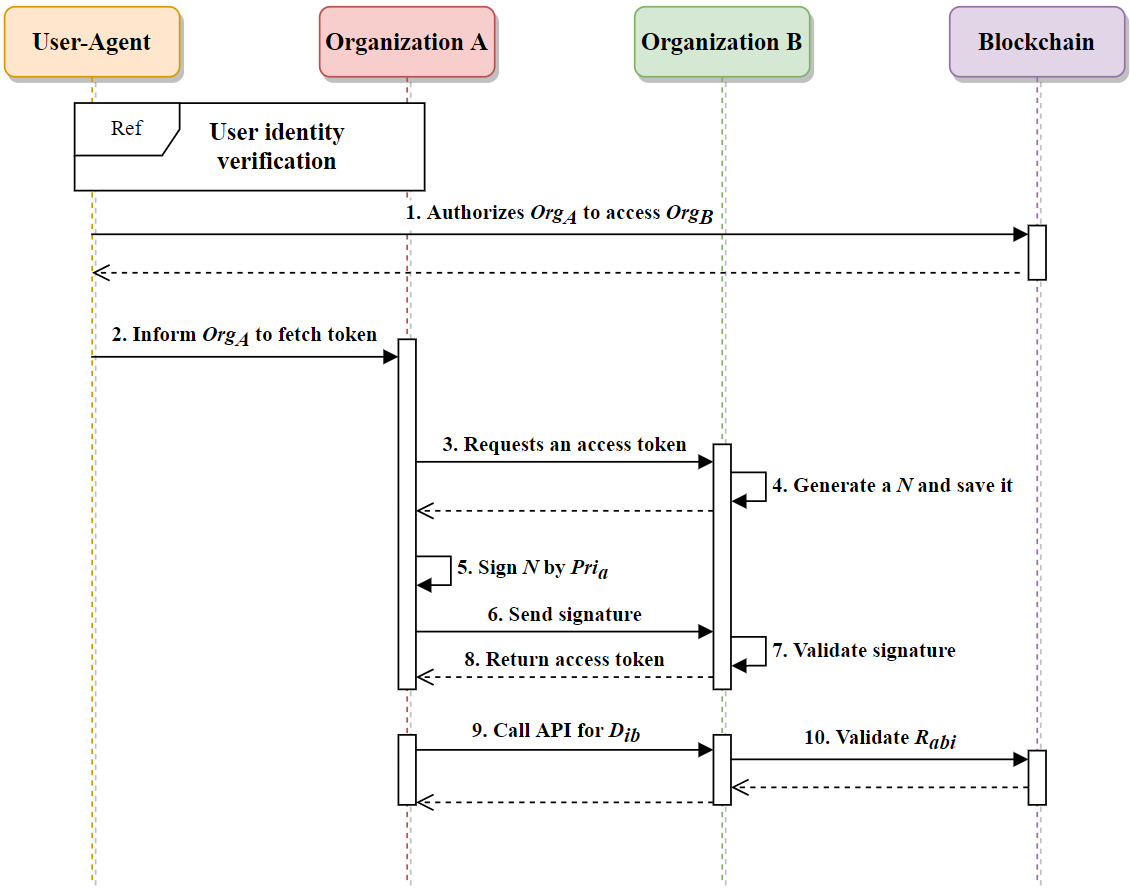
\includegraphics[height=!,width=1\linewidth,keepaspectratio=true]{figures/data_sharing.png}
        \caption{{\footnotesize Date Sharing flow}}
        \label{fig:dataSharing}
    \end{figure}

    The first step of this Figure~\ref{fig:dataSharing} shows that \(C_i\) authorize \(Org_A\) the access right to access the personal information stored in \(Org_B\). Any organizations are not involved in this authorization process, because web3.js library allows us to interact with the blockchain through the user-agent browser. The remaining steps are challenge-response authentication for obtaining an access token, one organization presents \(N\) and another organization must provide a valid signature, i.e., using private key to hash the specific \(N\). Thus, the organization which obtains access token can access user's data without authenticating again.
    
    \newpage